% !TEX encoding = UTF-8
% !TEX TS-program = pdflatex
% !TEX root = ../tesi.tex
% !TEX spellcheck = it-IT

%************************************************

%************************************************
\color{red}
Il sistema

-Componenti:

1. Data Cleaning;

2. NLP;

3. Information extraction and entity linking;

4. Clustering:

	- Similarità semantica;
	
    - Similarità sintatica;
   
    - Composizione;
 			

\color{black}

Dato uno stream  di tweet (ordinato temporalmente), l'obiettivo  è quello di individuare dei "topic” o “event”. In letteratura, come già descritto nel capitolo \ref{cap:capitolo2}, esistono due principali metodologie : document-pivot e feature-pivot.
In questo lavoro di tesi, è stata adottata la prima metodologia, l'obiettivo è quindi suddividere lo stream in cluster, tali che ciascuno di essi corrisponda a tutti i tweet relativi ad un \lq\lq evento\rq\rq.  
La definizione di evento utilizzata è quella utilizzata per il Topic Detection and Tracking (TDT) \cite{Allan:2002:TDT:772260} :
In seguito sono descritte in maniera più dettagliata tutte le fasi eseguite.
\begin{figure}[h]
    \centering
    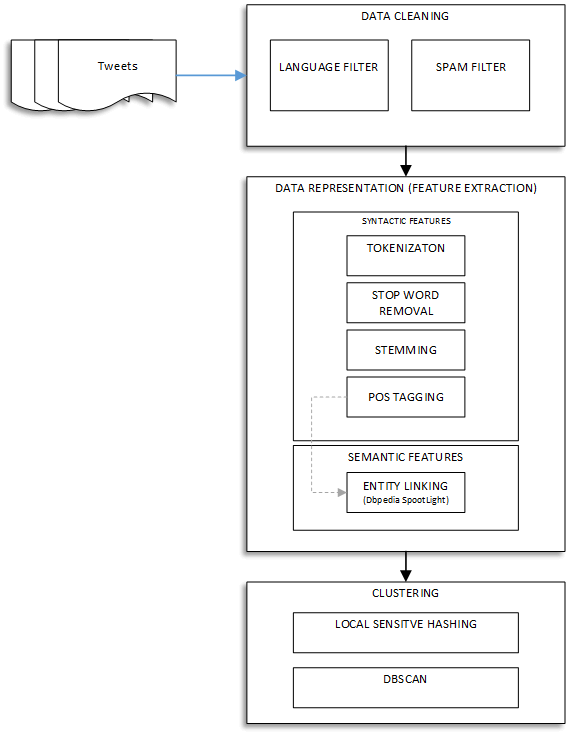
\includegraphics[width=0.6\textwidth]{diagrammaComponenti}
    \caption{Principali componenti del sistema}
    \label{fig:diagrammaComponentiSistema}
\end{figure} 


\section{Data Cleaning: Preprocessing}

Il preprocessing è uno step essenziale per qualunque task di text-mining, quando si ha a che fare con testo derivante dai social media come twitter, tale step diviene di vitale importanza a causa delle caratteristiche dei tweet. In Twitter gli utenti spesso usano slang, abbreviazione e talvolta coniano nuovi termini mai usati 
\`E dunque necessaria una fase accurata di preprocessing per il testo dei tweet prima di poter eseguire qualsiasi modellazione su di essi. 

Il primo passo in questa fase è la rimozione di quelle feature testuali legate ai tweet come:
\begin{itemize}
\item \emph{url:} dal testo sono eliminati tutti i riferimenti a url o media  
\item \emph{@-mentions:} vengono eliminate tutte le mentions ad altri utenti
\item  \emph{\#hashtag:} Per quanto riguarda gli hashtag viene solo eliminato il caratattere   \#   poiché fossero eliminati si potrebbe perdere della semantica dal testo.
Inoltre spesso nei tweet gli hashtag sono composizioni di più parole dove ciascuna parola inizia con una lettera maiuscola (camel Case), come ad esempio \#StopBombingGaza. Gli hashtag che si presentano nella forma su descritta verranno suddivisi nelle parole che di cui sono composti (\#StopBombingGaza $\rightarrow$ Stop Bombing Gaza).
\item \emph{RT:} per i retweet viene considerato il testo del tweet originale.
\end{itemize}
Per il primo passo non è necessaria alcuna fase di parsing del testo poiché tutte queste informazioni sono fornite dalle api di twitter sotto forma di dati strutturati\footnote{nell attributo entities del tweet}.

Molto spesso i tweet sono composti da keywords appartenenti a lingue diverse o contengono caratteri speciali, per tale motivo saranno eliminati tutti i non latin characters \cite{DBLP:conf/msm/BellaachiaA14} . 
 Tramite apposita espressione regolare vengono identificati ed eliminate le emoticons presenti nel testo.
 Una volta terminate queste operazioni di normalizzazione sono stati eseguite due operazioni di filtering:
 \begin{itemize}
 \item language-filtering sono stati considerati solo i tweet in lingua inglese
 utilizzando una libreria open-source scritta in java \footnote{https://code.google.com/p/language-detection/}.
 \item spam-filtering attraverso delle regole euristiche sono stati scartati quei tweet che, potenzialmente, rappresentano spam
 \end{itemize}
 
  
 
Per filtrare  quei tweet che rappresentano potenzialmente dello spam, sono state adottate delle regole empiriche:   \cite{Benevenuto10detectingspammers}
    \begin{itemize}
	\item tweet con più di tre hashtag
	\item tweet con più di due url
	\item tweet con più di tre user-mentions
	\end{itemize}
 


\section{Data Representation} 
Per poter applicare gli algorimi di machine learning è necessario rappresentare gli item attraverso vettori di feature.
I tweet saranno rappresentati come vettori, utilizzando il Vector space Model \cite{Salton:1989:ATP:77013}. 
Il Vector Space Model (VSM), in italiano Modello a Spazio Vettoriale, è una modellazione matematica per documenti testuali che si basa sull'assunzione che il significato dei documenti possa essere rappresentato dai termini che compongono il documento stesso. 
L'intero corpus di documenti, può essere quindi considerato come una matrice $A \in \mathbb{R}^{mxn}$, dove $m$  indica il numero dei termini distinti nel dizionario, $n$  il numero dei documenti 
La figura \ref{fig:vsm}  mostra una possibile rappresentazione in uno spazio vettoriale a tre dimensioni (ovvero vi sono solo tre termini) di tre documenti.

In questo modello, ciascuna dimensione dei vettori corrisponde ad un termine distinto, e sarà diversa da zero se il termine compare nel documento: i singoli valori $a_{ij}$ della matrice rappresentano il peso
assunto dal i-esimo termine nell’j-esimo documento.

 Questo peso può essere assegnato in base a  diversi schemi di pesatura, ed è solitamente funzione della frequenza del termine nello specifico documento e di altri fattori, mentre assume valore 0 in assenza del
termine nel documento. Di conseguenza questi vettori sono altamente dimensionali, e molto sparsi dato che i tweet sono composti al più da 140 caratteri. 

\begin{figure}[h]
    \centering
    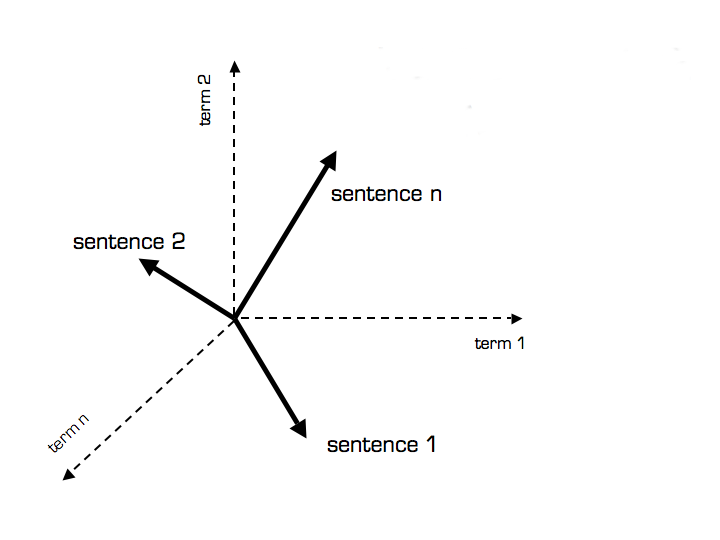
\includegraphics[width=0.6\textwidth]{vector_space}
    \caption{Esempio di documenti in uno spazio vettoriale.}
    \label{fig:vsm}
\end{figure}  


Il metodo di pesatura più utilizzato è quello del TF-IDF (Term Frequency-Inverse Document Frequency).
Dato una un termine  $t$, di un documento (tweet) $d$, in una collezione di documenti $D$
che è definita come  
\begin{equation}
tf-idf(t,d, D) =  tf(t,d)\cdot idf(t,D)
\end{equation}
La Term Frequency $tf(w,t)$ è dalla frequenza del termine all'interno del documento. Si presume, che un termine     ripetuto molte volte in un documento, sia molto indicativo del concetto che tale documento vuole esprimere.
Tuttavia vi sono termini che compaiono molto frequentemente in tutti i documenti (come congiunzioni. avverbi che hanno un basso potere informativo).
Per  mitigare questo effetto, viene utilizzato l'Idf che è definito come il logaritmo del rapporto fra numero totale dei documunti nel corpus, e il numero di documenti che contiene il termine $t$.
\begin{equation}
idf(t, D) =  \log \frac{|D|}{|\{d \in D: t \in d\}|}
\end{equation}
L'Inverse Document Frequency   indica la quantità di informazione di un dato termine, ovvero stabilisce se un termine è comune o meno all'interno del corpus. Più il termine è comune minore sarà la sua informazione. 
Poichè si utilizza il logaritmo, se un termine compare in tutti i documenti, il suo valore di Idf sarà pari a 0.

\subsection{Feature sintattiche}
Per poter trasformare il testo in vettori, sono state svolte delle operazioni di Natural Language Processing come:
\begin{enumerate}
\item \textbf{Tokenization}: In questa fase il testo viene suddiviso in unità atomiche dette \emph{token}
\item \textbf{Stop-Word removal}: Rimozione delle parole più comuni nel lessico
\item \textbf{Stemming}: Riduzione di ciascuna parola alla sua radice detta \emph{tema}
\item \textbf{Pos Tagging}: Ad ogni parola viene etichettata con la sua categoria lessicale (Part of Speech).
\end{enumerate}
\subsubsection{Tokenization}

La \emph{Tokenizzazione} è il primo passo di elaborazione di un sistema di Natural Language
Processing. Consiste nella separazione del flusso di caratteri che compone il testo
in input in una serie di elementi atomici detti \emph{token}. I token rappresentano le
unità minime di caratteri consecutivi e possono essere parole, spazio, simboli di
interpunzione e numeri. Sebbene questa operazione di suddivisione in token 
sembrare banale, presenta alcune problematiche. La semplice suddivisione in base allo spazio Suddividere non è sufficiente poiché in molti casi non
ci sono spazi che separano le parole dalla punteggiatura, ci sono sequenze di caratteri senza spazi al loro interno che rappresentano due distinti token (come ad esempio parole precedute da articolo con l'apostrofo, o banalmente parole virgolettate o all'interno di parentesi), esistono sequenze di caratteri. Esistono inoltre molte differenze nelle convenzioni ortografiche, ad esempio nelle date o nei numeri. 
Le tecniche per risolvere questi problemi prevedono l'uso di euristiche ed  espressioni regolari.
 
\subsubsection{Stop-Word Removal}

Le Stop Word sono parole che vengono individuate e filtrate o rimosse all'interno del processo di Natural Language Processing.
Parole come "the", "above", "for" non hanno nessun potere discriminativo all'interno di un documento, rimuoverle ha un vantaggio duplice: da un lato diminuisce la complessità del documento stesso, dall'altro evita che venagano in seguito considerati come simili dei documenti che contengono queste parole.
Generalmente, queste stop-word, sono contenute in una lista, la stop word list, che può contenere diversi tipi di parole a seconda degli obiettivi dell'applicazione. Solitamente vengono inserite nella lista le parole a più alta frequenza e dunque meno discriminanti, di un certo linguaggio, individuabili dunque all'interno delle categorie chiuse del discorso e tra le parole a maggiore frequenza
delle altre categorie, come ad esempio verbi ausiliari o parole molto generiche. In questo lavoro è stata utilizzata una lista contenente le classiche stopword per la lingua inglese \footnote{http://www.ranks.nl/stopwords}, a cui sono state aggiunte però
delle stopword specifiche per Twitter come: "Retweet","favorite","dm".
\subsubsection{Stemming}
Lo Stemming è il processo di riduzione della forma flessa o derivata di una parola alla sua radice detta \emph{tema}. 
Non è necessario che il tema corrisponda ad una valida radice morfologica, ma è utile che tutte le inflessioni o le derivazioni della parola
vengano ricondotte ad un unico tema, al fine di ridurre complessivamente lo spazio delle parole. 

 Ciò che materialmente gli algoritmi eseguono è la rimozione dei suffissi delle parole, che possono essere enclitici, ovvero essere particelle attaccate alla radice, flessioni che eseguono le declinazioni grammaticali di una parola di una certa categoria e derivazioni che cambiano categoria grammaticale o modificano il significato  

\subsubsection{Pos-Tagging}
 
Il Part of Speech Tagging consiste nell'associare a ciascuna parola nel testo, un'etichetta che si riferisce ad una parte del discorso o categoria lessicale in una frase (nome, pronome,verbo), basandosi sia sulla sua definizione che sul  suo contesto, ovvero la sua associazione rispetto alle parole adiacenti e correlate all'interno di una frase, di un periodo o di un paragrafo.
Esistono vari insiemi di categorie lessicali, i più utilizzati solo il Penn Treebank \footnote{https://cs.nyu.edu/grishman/jet/guide/PennPOS.html} e il Multext\footnote{http://universaldependencies.org/tagset-conversion/sl-multext-uposf.html}.
La tabella \ref{tab:PosTags} mosta un esempio di categorie lessicali (Part of Speech Tags) secondo il Penn Treebank.
La difficoltà del task di Part of Speech Tagging è data nell'ambiguità dell'assegnazione di una specifica etichetta ad una parola, poiché ogni parola può essere
etichettata in diversi modi, potendo essa appartenere a diverse categorie lessicali in base al contesto in cui compare 
Gli algoritmi utilizzati per il Part of Speech Tagging sono principalmente di due
categorie:
\begin{enumerate}
\item \textbf{Basati su regole}  di trasformazione, che impostano le etichette più probabili
per le parole ambigue e successivamente applicano una serie di trasformazioni
apprese da un dataset etichettato per raffinarne i risultati 
\item \textbf{Stocastici} la maggior parte basati su Hidden Markov Model,
che, dopo aver etichettato le parole certe, massimizzano la probabilità che una sequenza di parole abbia una determinata sequenza di etichette utilizzando l'algoritmo di Viterbi \cite{Ryan:1993:VA:901051}.
\end{enumerate}
\begin{table}[]
\centering
\caption{esempio di pos Tags di Penn TreeBank}
\label{tab:PosTags}
\begin{tabular}{ll}
\hline
 \textbf{Tag}& \textbf{Descrizione}\\ \hline
\texttt{CC}  & {Cordinate Conjunction}  \\ \hline
\texttt{CD}  & {Cardinal number}  \\ \hline
\texttt{CC}  & {Cordinate Conjunction}  \\ \hline
\texttt{NN}  & {Noun, singular or mass}  \\ \hline
\texttt{NNS}  & {Noun, plural}  \\ \hline
\texttt{NNP}  & {Proper noun, singular}  \\ \hline
\texttt{VB}  & {Verb, base form}  \\ \hline
\texttt{VBD}  & {Verb, past tense}  \\ \hline
\texttt{JJ}  & {Adjective}  \\ \hline
\texttt{PRP}  & {Personal pronoun}  \\ \hline
\end{tabular}
\end{table}
\subsection*{ }
Le prime tre fasi di estrazione di feature sintattiche (tokenizzazione, rimozione stopword e stemming) sono state implementate utilizzando le API di Apache Lucene \footnote{https://lucene.apache.org/core/}.

In particolare, per la prima fase di \emph{Tokenization}  è stata adottata la classe \emph{StandardTokenizer}. Questa classe segmenta il testo in token, seguendo le regole dell'algoritmo Unicode Text Segmentation \footnote{http://unicode.org/reports/tr29/}. 
Una volta ottenuti i token, questi vengono innanzitutto convertiti in minuscolo, e successivamente vengono filtrate le stopord.
Per la riduzione dei token alla radice (Stemming), è stata utilizzata la classe \emph{KStemFilter} che implementa lo stemming descritto nel lavoro di Krovetz \cite{Krovetz:1993:VMI:160688.160718}.

Per la fase di pos-tagging invece, è stato adottato il pos-tagger fornito da Stanford \cite{Toutanova:2000:EKS:1117794.1117802} che rientra nella categoria degli algoritmi stocastici. In particolare questo algoritmo è stato utilizzato in combinazione con un modello di training, costruito a partire da un dataset di tweets \cite{GateModelTagger} fornito dall'università di Sheffield.



A partire da queste feature-sintattiche, saranno definiti i pesi di ciascun token all'interno di un tweet.
In particolare, il peso di un termine $t$ di un tweet sarà dato da:
\begin{equation}
tf-idf_t=tf(t)\ log\frac{N_t}{df(w)}boost(w)
\end{equation}
 Risulta fondamentale assegnare un boost ovvero un peso maggiore a determinati termini poiché, a causa del limite dei 140 caratteri, il $tf$ di ciascuna keyword è solitamente pari a 1. 
\begin{equation*}
boost(t):=\begin{cases}
2.0 & \text{se $t$ è un hashtag, on un Proper Nooun}\\
1& \text{altrimenti.}
\end{cases}
\end{equation*}
Solitamente uh hashtag ha un alto potere informativo all'interno di un tweet inoltre nel lavoro di  Phuvipadawat \cite{Phuvipadawat:2010:BND:1913791.1913911}  il boost maggiore per i poper-noun ha prodotto risultati migliori.





\subsection{Feature Semantiche}
\subsubsection{Entity Linking} 
Nell'elaborazione del linguaggio naturale, l'attività di Entity Linking (detta anche Named Entity Disambiguation NED, o named entity recognition and disambiguation (NERD)), ha l'obiettivo di identificare delle entità menzionate nel testo. Ad esempio, dato il testo \emph{\lq\lq Paris is the capital of France \rq \rq} l'obiettivo è quello di stabilire che   "Paris" si riferisce alla città piuttosto che a Paris Hilton o a qualsiasi altra entità.
Questa attività differisce dal Named Entity Recognition, poiché in quest'ultima vengono soltanto identificate le occorrenze o menzioni ad entità ma non viene stabilito quali siano.
L'attività di Entity Linking richiede necessariamente una base di conoscenza (Knowledge Base) contenente tutte le possibili entità che possono essere menzionate. La basi di conoscenza più utilizzate a tal fine sono  Wikipedia, o la versione come linked open data: DBpedia.

Generalmente questo task consiste può essere suddiviso in tre step:
\begin{enumerate}
\item \textbf{Spotting} a partire dal testo del documento viene identificato un insieme di possibili citazioni, e per ciascuna di queste viene ritrovata una lista di tutte le possibili entità.
\item \textbf{Disambiguation} nel caso in cui ad una sotto stringa siano state associate più di un'entità, verrà scelta una sola.
\item \textbf{Ranking}: solitamente tutte  le entità annotate sono ordinate in base ad un qualche criterio come ad esempio il grado di confidenza di ciascuna annotazione.
\end{enumerate}

\subsubsection{Dbpedia Spootlight}
Spotlight è un progetto di ricerca nato nel giugno del 2010 all'interno della Freie Universität Berlin . Il gruppo di sviluppatori è costituito da Pablo Mendes, Max Jakob e Jo Daiber ed è supervisionato da Chris Bizer, il fondatore del progetto DBpedia, nonché figura di grande rilievo a livello internazionale nel campo del Semantic Web. Spotlight è finanziato dalla Commissione Europea at-
traverso il progetto LOD2 – Creating Knowledge out of Linked Data \footnote{www.semantic-web.at/lod2-creating-knowledge-out-interlinked-data} .
DBpedia Spotlight \cite{isem2013daiber}  si propone come uno strumento per annotare automaticamente le
menzioni di entità di DBpedia all'interno di testi e quindi per collegare dati non strutturati ai repository della Linked Open Data Cloud.
Una delle più grandi sfide di questo task è dato dall'ambiguità del linguaggio naturale, spesso uno stesso nome di entità può riferirsi a più di una risorsa DBpedia. (es: \emph{Washington} può riferirsi alla città  , allo stato o al presidente).
Pone grande rilevo al problema della WSD, cercando di offrire all'utente una soluzione molto parametrizzabile che incontri le sue esigenze a livello sia di precisione che di recall.
Utilizzando DBpedia come base di conoscenza, questo tool ha un ampio bacino di applicabilità, a differenza di altri sistemi esistenti dove le annotazioni sono ristrette ad un numero  limitato di tipologie \'E però possibile anche restringere il range di annotazioni ad
 un dominio più ristretto di tipologie di entità, indicando solo alcune classi  l'ontologia DBpedia di cui si desiderano delle annotazioni. O in alternativa si può fornire una query SPARQL, per estrarre annotazioni che soddisfino dei vincoli particolari, ad esempio, solo annotazioni che si riferiscono a politici in carica dal 2010 al 2012 di una data città.  (Persone,organizzazioni luoghi).
 


Uno dei maggiori punti di forza di questo tool è dato dalla sua flessibilità: è possibile fornire dei parametri al sistema in modo tale da soddisfare al meglio i propri requisiti.
In particolare è possibile specificare come parametri addizionali\footnote{oltre al testo}:
\begin{itemize}
\item \textbf{Tipologie di risorse} è possibile fornire un insieme di classi DBpedia di cui si desiderano annotazioni, es:
si desiderano solo annotazioni  geografiche si può fornire la classe \emph{dbpedia:Place}.  alternativa è possibile fornire nuna query SPARQL per esprimere dei vincoli più sofisticati (es  tutte le chiese di Roma) .
\item \textbf{Importanza della risorsa-supporto}: In molti casi è desiderabile che molto rare o molto specifiche non siano restituite affatto. Un indicazione dell'importanza di una risorsa è data dal numeri di \emph{in-link}. \'E possibile specificare il numero minimo di in-link di una risorsa da annotare.
\item \textbf{Confidenza}: si può fornire un fattore di confidenza che varia nell'intervallo $[0,1]$  che indica il grado di sicurezza dell'annotazione, tenendo conto sia della similarità del testo rispetto all'annotazione
\end{itemize}
 

\begin{figure}[h]
    \centering
    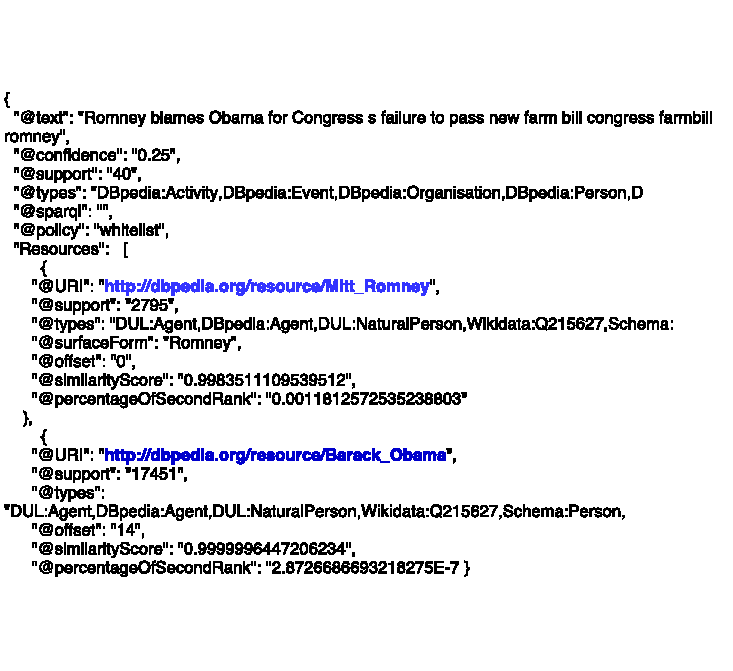
\includegraphics[width=0.8\textwidth]{annDBPEDIA.pdf}
    \caption{Esempio di output del processo di annotazione di DBpedia Spootlight}
    \label{fig:dbpediaAnn}
\end{figure}   
DBpedia Spootlight è reso disponibile sia come Web Service sia RESTful che SOAP su un server pubblico. Se si desiderano dei bassi tempi di latenza ed un servizio con maggiore affidabilità è anche possibile lanciare il web-service su un proprio server.

La figura \ref{fig:dbpediaAnn} mostra un esempio di risposta in formato JSON del web-serice: le annotazioni sono sono restituite sotto forma di array di oggetti \emph{Resources}.
Ciascun oggetto di tale array costituisce una singola annotazione di cui viene indicato :
\begin{itemize}
\item \textbf{@URI}: URI della risorsa DBpedia associata
\item \textbf{@support}: numero di inLink della risorsa DBpedia
\item \textbf{@types}: classificazione della risorsa 
\item \textbf{@surfaceForm}: sottostringa del testo cui si riferisce l'annotazione
\item \textbf{@similarityScore}: rilevanza della risorsa rispetto alla surfaceForm, e varia fra 0 e 1.
\item \textbf{@percentageOfSecondRank}: nel caso in cui ad una surfaceForm siano state associate più di un'entità, queste vengono ordinate in base alla rilevanza.
Il fattore \emph{percentageOfSecondRank}  indica il rapporto di  della similarità  fra la risorsa classificata come seconda e la prima. Più è alto maggiore è l'ambiguità dell'annotazione.
\end{itemize}


Poiché questo task di annotazione è stato svolto su posti di Twitter  ulteriori problematiche dovute alle caratteristiche dei tweets.
Molto spesso nei tweets quando si condivide un immagine, o un video vi sono riferimenti ad altre social network es: Facebook, Instangram, Youtube.
Questi social network sono correttamente identificati  da DbpediaSpootlight all'interno del testo, ma in questo contesto non hanno nessuna valenza semantica.  A tal fine è stata definita una lista di quelle risorse dpbedia non desiderate, una sorta di black-list per filtrare queste annotazioni.


Inoltre è stato riscontrato in maniera empirica che il tool DBepdai Spootlight tende ad annotare  sotto stringhe anche quando queste sono utilizzate come aggettivi (es Russian   Russia).
Il risultato della fase di pos-tagging è stato quindi utilizzato per filtrare solo quelle annotazioni che contengono almeno un nome. 





 Ciò permette di arricchire la rappresentazione testuale andando a lenire i classici problemi di ambiguità del linguaggio naturale come polisemia e sinonimia.  





Annotare il testo con DBpedia URIs permette di sfruttare la base di conoscenza di DBpedia per poter determinare la correlazione semantica fra due termini. 


 
 

\section{Semantic Annotation}





Avendo due risorse DBpedia è possibile definire una funzione di distanza, che sfrutti la base di conoscenza di DBpedia.  
Milne e Witten \cite{Milne08aneffective} hanno utilizzato gli hyperlink delle pagine Wikipedia per poter definire la correlazione fra due articoli wikipedia (e quindi due risorse dbpedia): date due risorse $a,b$, possiamo definire una \emph{Normalized DBpedia Distance (NDD)} come segue:
\begin{equation} \label{eq:normalized_dbpedia_distance}
NDD(a,b):=\begin{cases}
\frac{\log(max\{|A|,|B|\})-log( |A \cap B|\})}{log(N)-\log(min\{|A|,|B|\})} & \text{se $A \cap B \neq \emptyset $  ,}\\
1 & \text{altrimenti}\\
\end{cases}
\end{equation}
 $A$ e $B$  sono gli insiemi delle risorse DBpedia che hanno un link rispettivamente verso $a$ e $b$, mentre $N$ è il numero totale di risorse in DBpedia. Questa distanza varia nell'intervallo [0,1] dove 1 sta ad indicare che non vi è nessuna correlazione fra i due concetti, mentre 0 indica che i due concetti hanno lo stesso significato. L'idea alla base, è che due risorse saranno simili se esiste una terza che ha un link verso entrambe.
 


 sono necessari ulteriori steps per filtrare 
 
 
\section{Clustering}

 \begin{figure}[h]
    \centering
    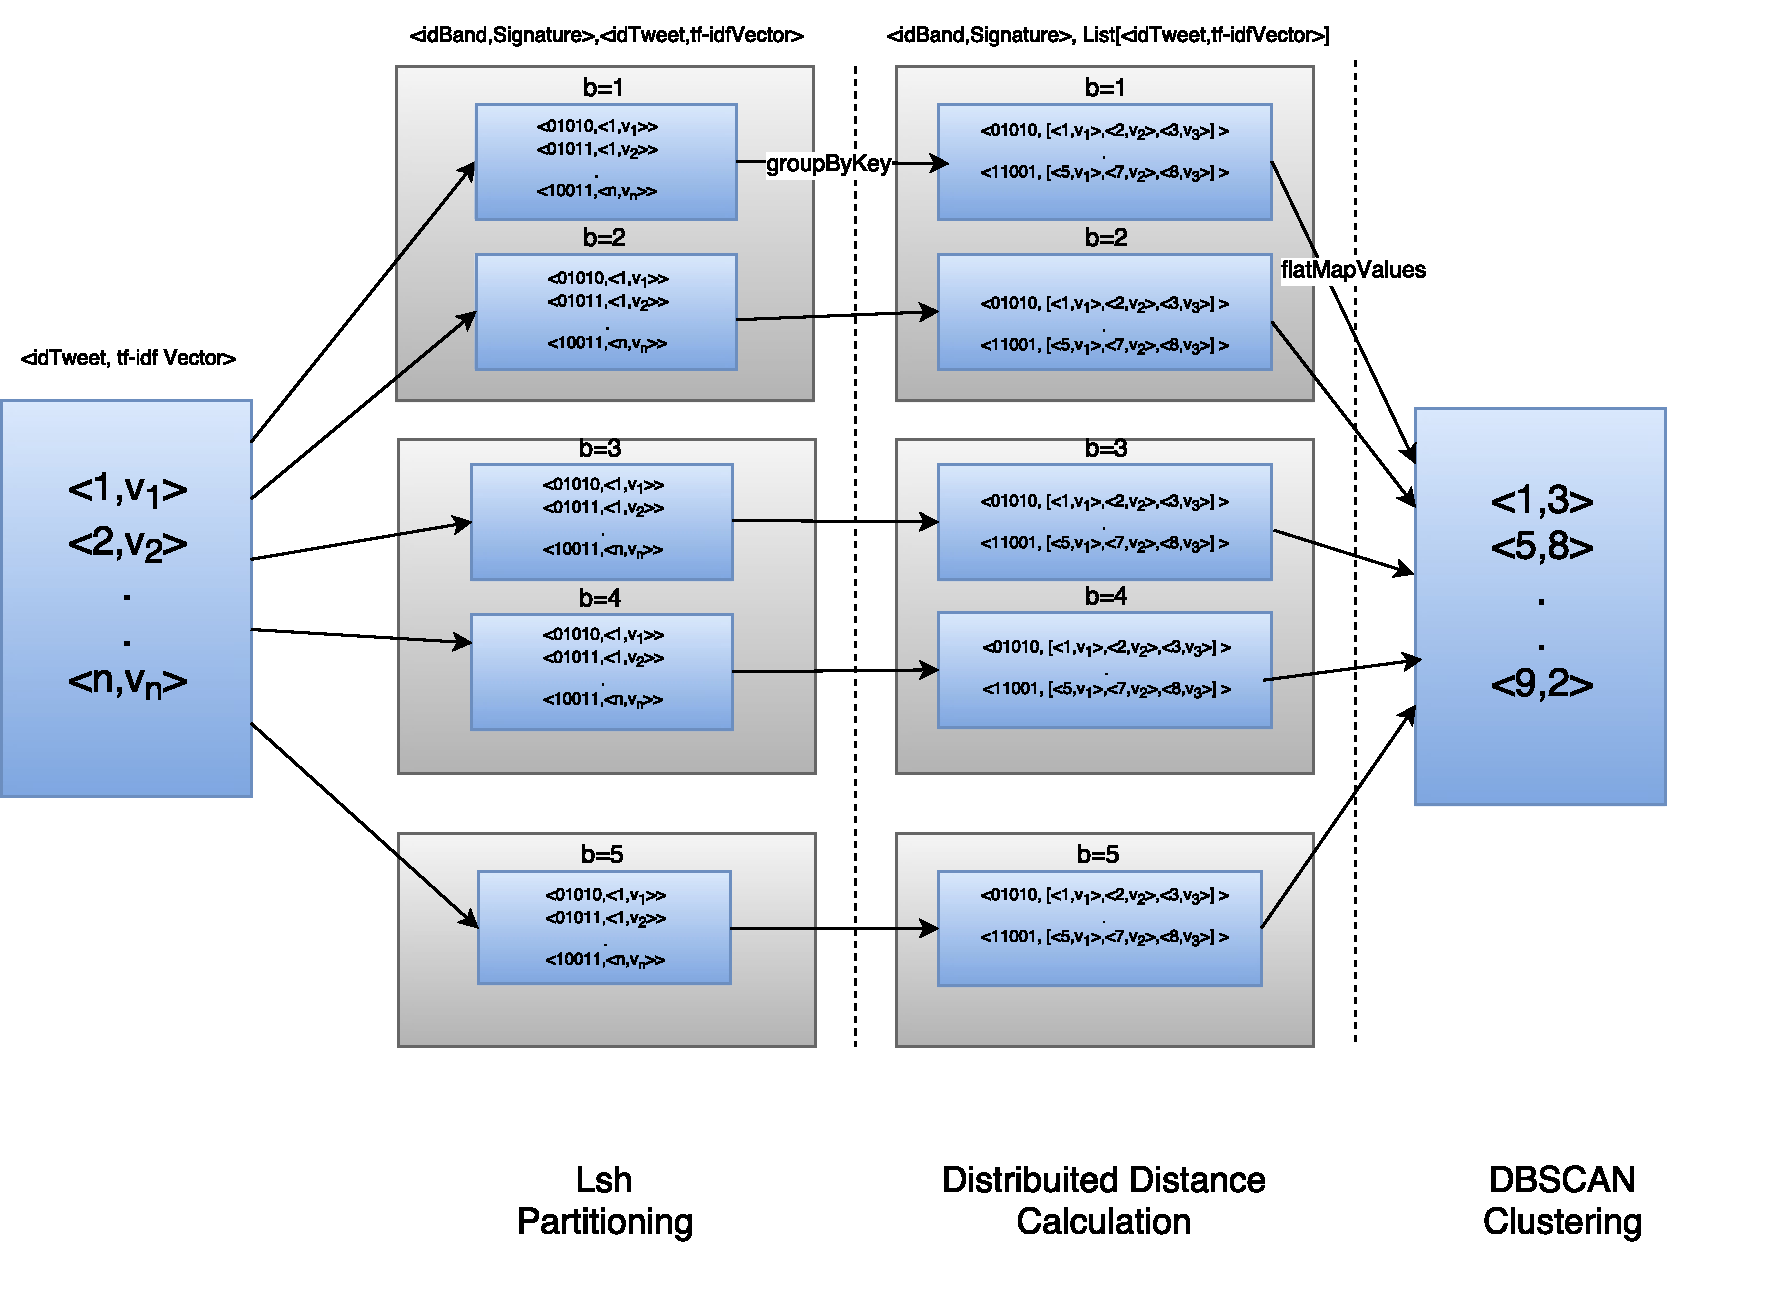
\includegraphics[width=0.8\textwidth]{clusteringWithSpark.pdf}
    \caption{esecuzione distribuita}
    \label{fig:clusteringWithSpark}
\end{figure}  


L'algoritmo di clustering utilizzato è  Dbscan poiché può gestire bene il rumore e non necessita di parametri come il numero di cluster a priori. La distanza utilizzata si basa sia sulla rappresentazione tf-idf del tweet sia sui DBpedia URIs estratti :
\begin{equation}
dist(a,b)=1- timeSim(a,b)\,\frac{textSim(a,b)+semanticSim(a,b)}{2}
\end{equation}
La similarità testuale è data dalla similarità del coseno fra i vettori tf-idf dei due tweet:
\begin{equation*}
textSim(a,b)=\frac{v_a \cdot  v_b}{||v_a||\:||v_b||}
\end{equation*}
 Anche il tempo di creazione dei tweet verrà preso in considerazione per valutarne la distanza, poiché anche se due tweet avessero un testo molto simile es \emph{“tonight  flashmob in central park”}, ma fossero pubblicati ad un mese di distanza, è molto inverosimile che si riferiscano al medesimo evento. Per tale ragione, è stata definita una similarità temporale  \footnote{d$_a$=\#days from the epoch of tweet $a$}
\begin{equation*} 
timeSim(a,b):=\begin{cases}
1-\frac{|d_a-d_b|}{31} & \text{se $|d_a-d_b|<31 $  ,}\\
0 & \text{altrimenti}\\
\end{cases}
\end{equation*}
Ad un tweet, tramite il processo di annotazione semantica, possono essere associate una nessuna o più risorse DBpedia,la distanza semantica sarà data dalla distanza degli insiemi di risorse associati ai due tweet valutata secondo la distanza definita in precedenza per le risorse DBpedia\ref{eq:dbpedia_semantic_distance}. La similarità fra un elemento $x$ e un insieme $Y$ è data da:
\begin{equation*}
	sim(x,Y)=sup\{1-DSD(x,y)\:| y\in Y \}
\end{equation*}

Dati due insiemi di risorse DBpedia $D_a,D_b$ la similarità fra i due insiemi sarà definita come: 
\begin{equation}
sim(D_a,D_b)=\frac{\sum\limits_{x \in D_a} sim(x,D_b)  }{|D_a|} 
\end{equation}

Questa funzione di similarità non è simmetrica,\footnote{se $D_a\subseteq D_b\Rightarrow sim(D_a,D_b)\neq sim(D_b,D_a) $}
Per ottenere una funzione simmetrica è sufficiente definirla come: 
\begin{equation*} 
semanticSim(a,b):= 
\begin{cases}
\frac{sim(D_a,D_b)+sim(D_b,D_a)}{2} & \text{se $D_a,D_b\neq \emptyset$ }\\
1& \text{altrimenti.}

\end{cases}
\end{equation*}
Se ad uno dei due tweet non è associata nessuna risorsa, la similarità semantica sarà pari ad uno, quindi la loro similarità sarà valutata  solo in base alla loro rappresentazione testuale.
Utilizzare una similarità semantica serve ad attenuare il problema della “fragmentation” di cui sono affetti i metodi document-pivot, ovvero utilizzando solo la similarità testuale molti eventi possono essere erroneamente suddivisi in più cluster.  Inoltre Petkos e Papadopoulus \cite{DBLP:conf/www/PetkosPK14}  hanno constato che se due tweet condividono uno stesso URL, o  un tweet e in reply all’altro, allora si riferiscono allo stesso topic/evento.
 
\begin{figure}
    \centering
    \begin{subfigure}[b]{0.45\textwidth}
        \centering
        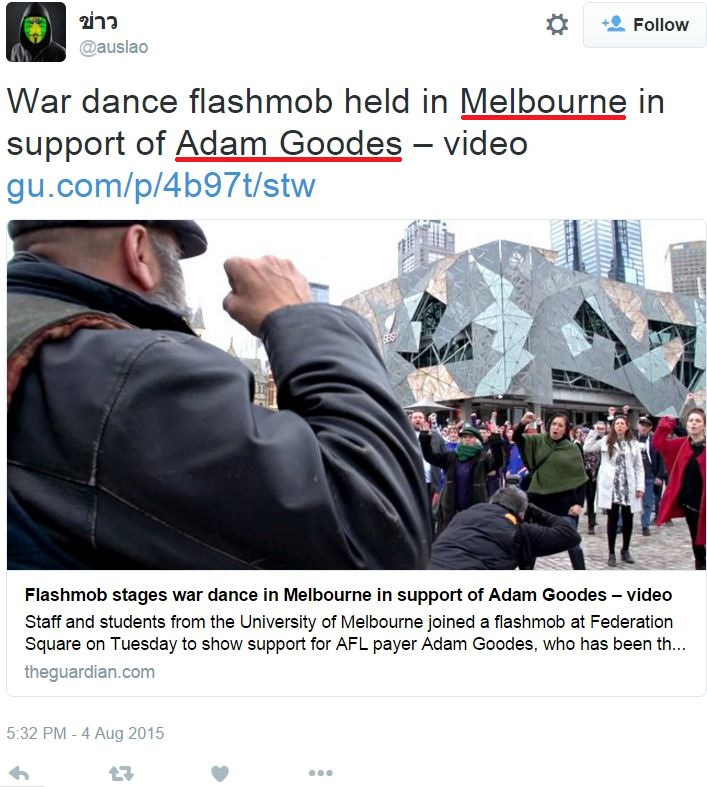
\includegraphics[width=\textwidth]{tweetA}
        \caption{}
        \label{fig:tweeta}
    \end{subfigure}
    \hfill
    \begin{subfigure}[b]{0.45\textwidth}
        \centering
        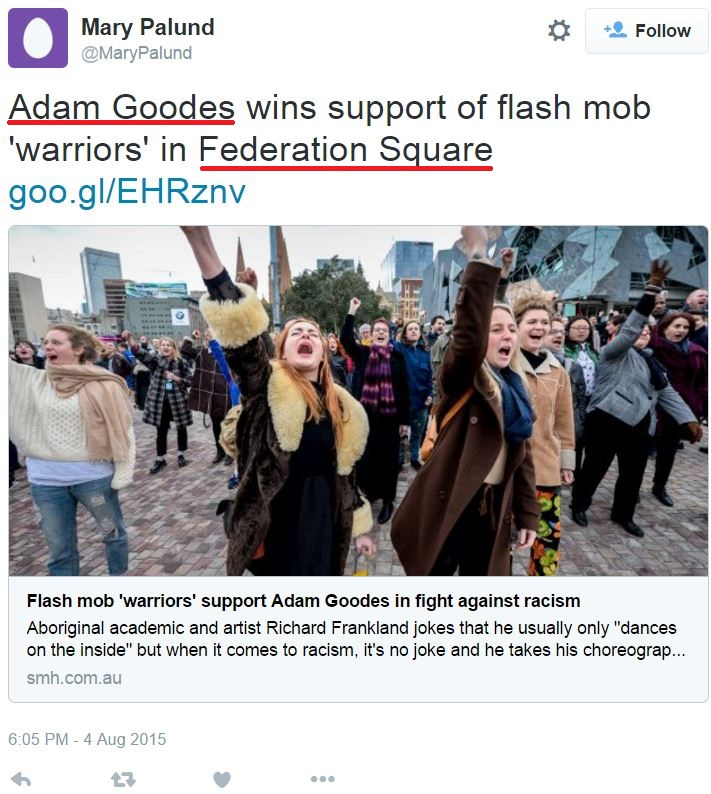
\includegraphics[width=\textwidth]{tweetB}
       \caption{}
        \label{fig:tweetb}
    \end{subfigure}
    \hfill
    
    \caption{Due tweet appartenti allo stesso cluster}
    \label{fig:twotweets}
\end{figure} 
Si considerino i tweet $a,b$ in figura \ref{fig:twotweets}:

\begin{itemize}
\item $textSim(a,b)=0.46$ 
\item $timeSim(a,b)=1.0$ i tweet sono stati pubblicati entrambi il 4/8/2015
\item $semanticSim(a,b):=\frac{sim(D_a,D_b)+sim(D_b,D_a)}{2} $



  $D_a=$\{ \textless\href{http://dbpedia.org/resource/Melbourne}{Melbourne}\textgreater, \textless\href{http://dbpedia.org/resource/Adam_Goodes}{Adam Goodes}\textgreater\}
  
  $D_b=$\{ \textless\href{http://dbpedia.org/resource/Adam_Goodes}{Adam Goodes}\textgreater, \textless\href{http://dbpedia.org/resource/Federation_Square}{Federation Square}\textgreater\}
  
\begin{align*}
 NSD(Melbourne,Adam Goodes)&=NDD(Melbourne,Adam Goodes)\\
 &= \frac{\log(max\{|A|,|B|\})-log(|A \cap B|)}{N-\log(min\{|A|,|B|\})}\\
 &= \frac{\log(643)-log(10)}{N-\log(138)}=0.367  
\end{align*} 
\begin{align*}
 NSD(Melbourne,Federation Square)&=\\
 =GeoDist(Melbourne,Federation Square)&=\\
 =CoordDist(Melbourne,Federation Square) &=0 \: \text{(poichè la distanza in km è 0.8)}
\end{align*}  
\begin{align*}
 NSD(Adam Goodes,Federation Square)=&\\
 NDD(Adam Goodes,Federation Square)&=1 \: \text{poichè} \: A \cap B=\emptyset
\end{align*} 

\begin{align*}
 sim(Melbourne,D_b)&=sup\{1-DSD(Melbourne,y)\:| y\in D_b \}\\
	&=sup\{(1-DSD(Melbourne,Adam Goodes)),\\
	&\:\:\:\:(1-DSD(Melbourne,Federation Square))\}\\
	&=sup\{(1-0.367),(1-0)\}=1	\\	  
 sim(Adam Goodes,D_b)&=sup\{1-DSD(Adam Goodes,y)\:| y\in D_b \}\\
	&=sup\{(1-DSD(Adam Goodes,Adam Goodes)),\\
	&\:\:\:\:(1-DSD(Adam Goodes,Federation Square))\}\\
	&=sup\{(1-0),(1-1)\}=1\\		 
sim(D_a,D_b) &=\frac{1+1}{2}=1 ,\: sim(D_b,D_a) :=\frac{1+1}{2}=1\\
&\implies semanticSim(a,b)=1
\end{align*}
\end{itemize} 
 \begin{align*}
dist(a,b)&=1- timeSim(a,b)\,\frac{textSim(a,b)+semanticSim(a,b)}{2}\\
&=1-\frac{0.46+1}{2}=0.269
\end{align*}

Se invece, $SemanticSim$ fosse definita come la media delle distanze fra tutte le possibili coppie fra i due insiemi avremmo: 

\begin{align*}
	semanticSim(a,b)&=\frac{\sum\limits_{x \in D_a} \sum\limits_{x \in D_b}  (1-NSD(x,y))}{|D_a||D_b|}=\\
	&=\frac{(1-0.36)+(1-0)+(1-0)+(1-1)}{4}=0.73
\end{align*}